%%%%%%%%%%%%%%%%%%%%%%%%%%%%%%%%%%%%%%%%%%%%%%%%%%%%%%%%%%%%%%%%%%%%%%%%%%%%%%%%
% Scenarios and Evaluation
% - Find a nice way to mention the scenario and how the visualization works
% - Probably want to divide up the discussion section for the study and expand
%   it a bit more.
% - Scenario ideas
%      > Spatial with lens 
%      > Toyota recall analysis 
%      > Comparison during car purchase ???
%%%%%%%%%%%%%%%%%%%%%%%%%%%%%%%%%%%%%%%%%%%%%%%%%%%%%%%%%%%%%%%%%%%%%%%%%%%%%%%%

\chapter{Scenarios and Evaluation}
In this chapter, we present several scenarios to show the possible uses cases
for our visualization. Following that, in the second section we present a
qualitative evaluation study of our system, discuss the study results and our
observations.

%%%%%%%%%%%%%%%%%%%%%%%%%%%%%%%%%%%%%%%%%%%%%%%%%%%%%%%%%%%%%%%%%%%%%%%%%%%%%%%%
\section{Scenarios}
We present three different scenarios to show how different facets of the
visualization can be used to analyze data and facilitate decision making tasks.
The first two are hypothetical scenarios and are used to demonstrate our system
functions: spatial exploration and making comparisons. In the third and last
scenario, we take a look at a real world event and see if the dataset reveals
any interesting facts surrounding the event.

 
\subsection{Spatial Exploration}
This scenario describes how a regular consumer, Larry, may use the 
visualization to research a problem. Larry has about three years of driving 
experience but does not know a lot about cars. Recently, while driving, he 
noticed a rattling sound coming from the passenger side of his vehicle. 
He decides to conduct some research on his own before taking the car back 
to the dealership.

Using the visualization, Larry filters the dataset to focus on his
vehicle model. Since Larry is not sure exactly where the noise came from, 
he uses the lens widget to focus on components near the front-passenger 
region. Using the lens, Larry can see that the suspension component has a
higher number of complaints registered against it than the other components 
in the focused area. Larry then selects the suspension component using 
the heatmap, and toggles the document widget so he can read through the 
actual complaint reports. After a few minutes of reading, Larry notes that
there are at least eight or nine reports that seemed to document similar noise 
issues and point to defective suspension setup. Larry decides that he 
should contact his dealership to have them check it out.

 
\subsection{Vehicle Comparison}
This scenario describes how our visualization may guide purchasing decisions.
Sara just accepted a job offer across town, and is looking to purchase a car 
for her commute. She previously had her mind settled on a used Honda Civic, 
but her friends have been saying good things about Nissan Sentra. With the 
visualization system, Sara uses the comparison function to compare Civic to 
Sentra, she then turns on the aggregation mode function so the visualization 
shows the system level view. 

Sara sees that engine and wheel components are both lightly shaded, which
indicates that neither one had serious issues regarding these sub systems.
However, she notices that there are dark green outlines around several
components, using the lens she identifies them as parts of the transmission subsystem. It seems like Sentra had
a much higher rate of transmission failure than Civic. Selecting the
transmission, Sara reads through several complaint reports, Sara then decides
that her original intuition about Honda Civic is correct.


\subsection{Retrospective Analysis}
In this scenario, we use our system to examine the Toyota recall. The Toyota 
vehicle recall happened between September 2009 to February 2010 and had to
do with defective brakes and accelerators. We are curious to see if there are
any patterns, in terms of leading or lagging indicators in the complaint data.
We set the time sliders to show 2009 and 2010 as seen in Figure \ref{figure:heatmap} 
and use the heatmap widget to observe for patterns.

The first thing we noticed is that the engine, usually one of the highest
occurring components in the complaint reports, no longer dominated
the visualization. Instead, two components pop out: brakes and accelerator.
A closer examination with the lens widget raised more questions.
The heatmaps show that there are two outlier months where a
huge amount of complaints were registered: February 2010 and March
2010, after the recall was announced. Perhaps the widely publicized
event triggered a loss in consumer confidence, which in turn led to an
over-reporting of problems. This is supported by the sharp drop-off
after March 2010.

% \subsection{Finding Causal and Related Issues}
% Curly is an automobile defect investigator, he is in the process of gathering
% information about a possible defect in the 2009 model of sedans. He leverage the
% NHTSA database as a data source for consumer initiated complaint reports. He
% enters the criteria one by one: manufacturer, model, make and the date range he
% wants to search for. After reviewing several dozen reports with brake issues he
% notices that there seem to be a trend emerging: over 50 percent of the reports
% read so far also mentions problems with the accelerator pedal. Thinking that
% there may be a connection between these two components Curly decides that he
% should widen his search criteria to include both accelerator and brakes.
% 
% Our system suggest causal relations by explicitly highlighting the related
% entities in text documents. Rather than having to account for related terms in
% his head, Curly can select the brake component in the visualization, which will
% high light all co-occurring entities, include the accelerator. A visual scan
% will reveal the high occurring, which Curly can select, and use the document
% panel to read the detailed complaint descriptions.


%%%%%%%%%%%%%%%%%%%%%%%%%%%%%%%%%%%%%%%%%%%%%%%%%%%%%%%%%%%%%%%%%%%%%%%%%%%%%%%%
\section{Evaluation}
We conducted an evaluation to see how the visualization is perceived and how
people perform analytical tasks. In order to create a realistic scenario, we
leveraged the vehicle complaint dataset. The study is framed around the idea of
analysing safety and reliability concerns. Our evaluation is based on how
participants interpret the visualization and  whether their decisions are
derived based on what the visualization is showing them. We also look at the process
participants go through to complete more open-ended tasks.

%Participants were evaluated on their
%interpretation of the visualization, as well as the process they go through to 
%complete complex scenarios. 

We have considered performance measures, in particular, against existing applications
that allow people to search and browse NHTSA dataset. However, as the application
interfaces are vastly different than ours, we did not believe such comparison would
be fair. Also, the tasks would be severely constrained to be possible on both
interfaces that they may not yield any meaningful results.

%nor would it yield any meaningful results.

%Our hypothesis states that when it comes to visualizing data involving physical
%objects, people may be able to communicate and gain better insights if we
%present the visualization to match real world entities. We take the first steps
%in evaluating our hypothesis by studying how people respond to our \threed
%interface and if they can use our visualization to solve analytical tasks. Our
%primary concerns are not whether the visualization is more efficient than
%conventional interfaces, rather, we focus on the type of questions that can be
%answered by our software as well as the user-experiences of using our prototype.


\subsection{Methodology}
We recruited 12 participants from the student population. All participants had some
type of experience with touch interfaces such as tablets and smart phones. Six 
had some experiences with \threed interfaces, through games or CAD-like
software. For experiences relating to the automotive domain, two participants
currently own a vehicle, while seven had previously investigated safety issues in
some way. 
 
    % === Figure === 
	\begin{figure}
	 \centering  
	 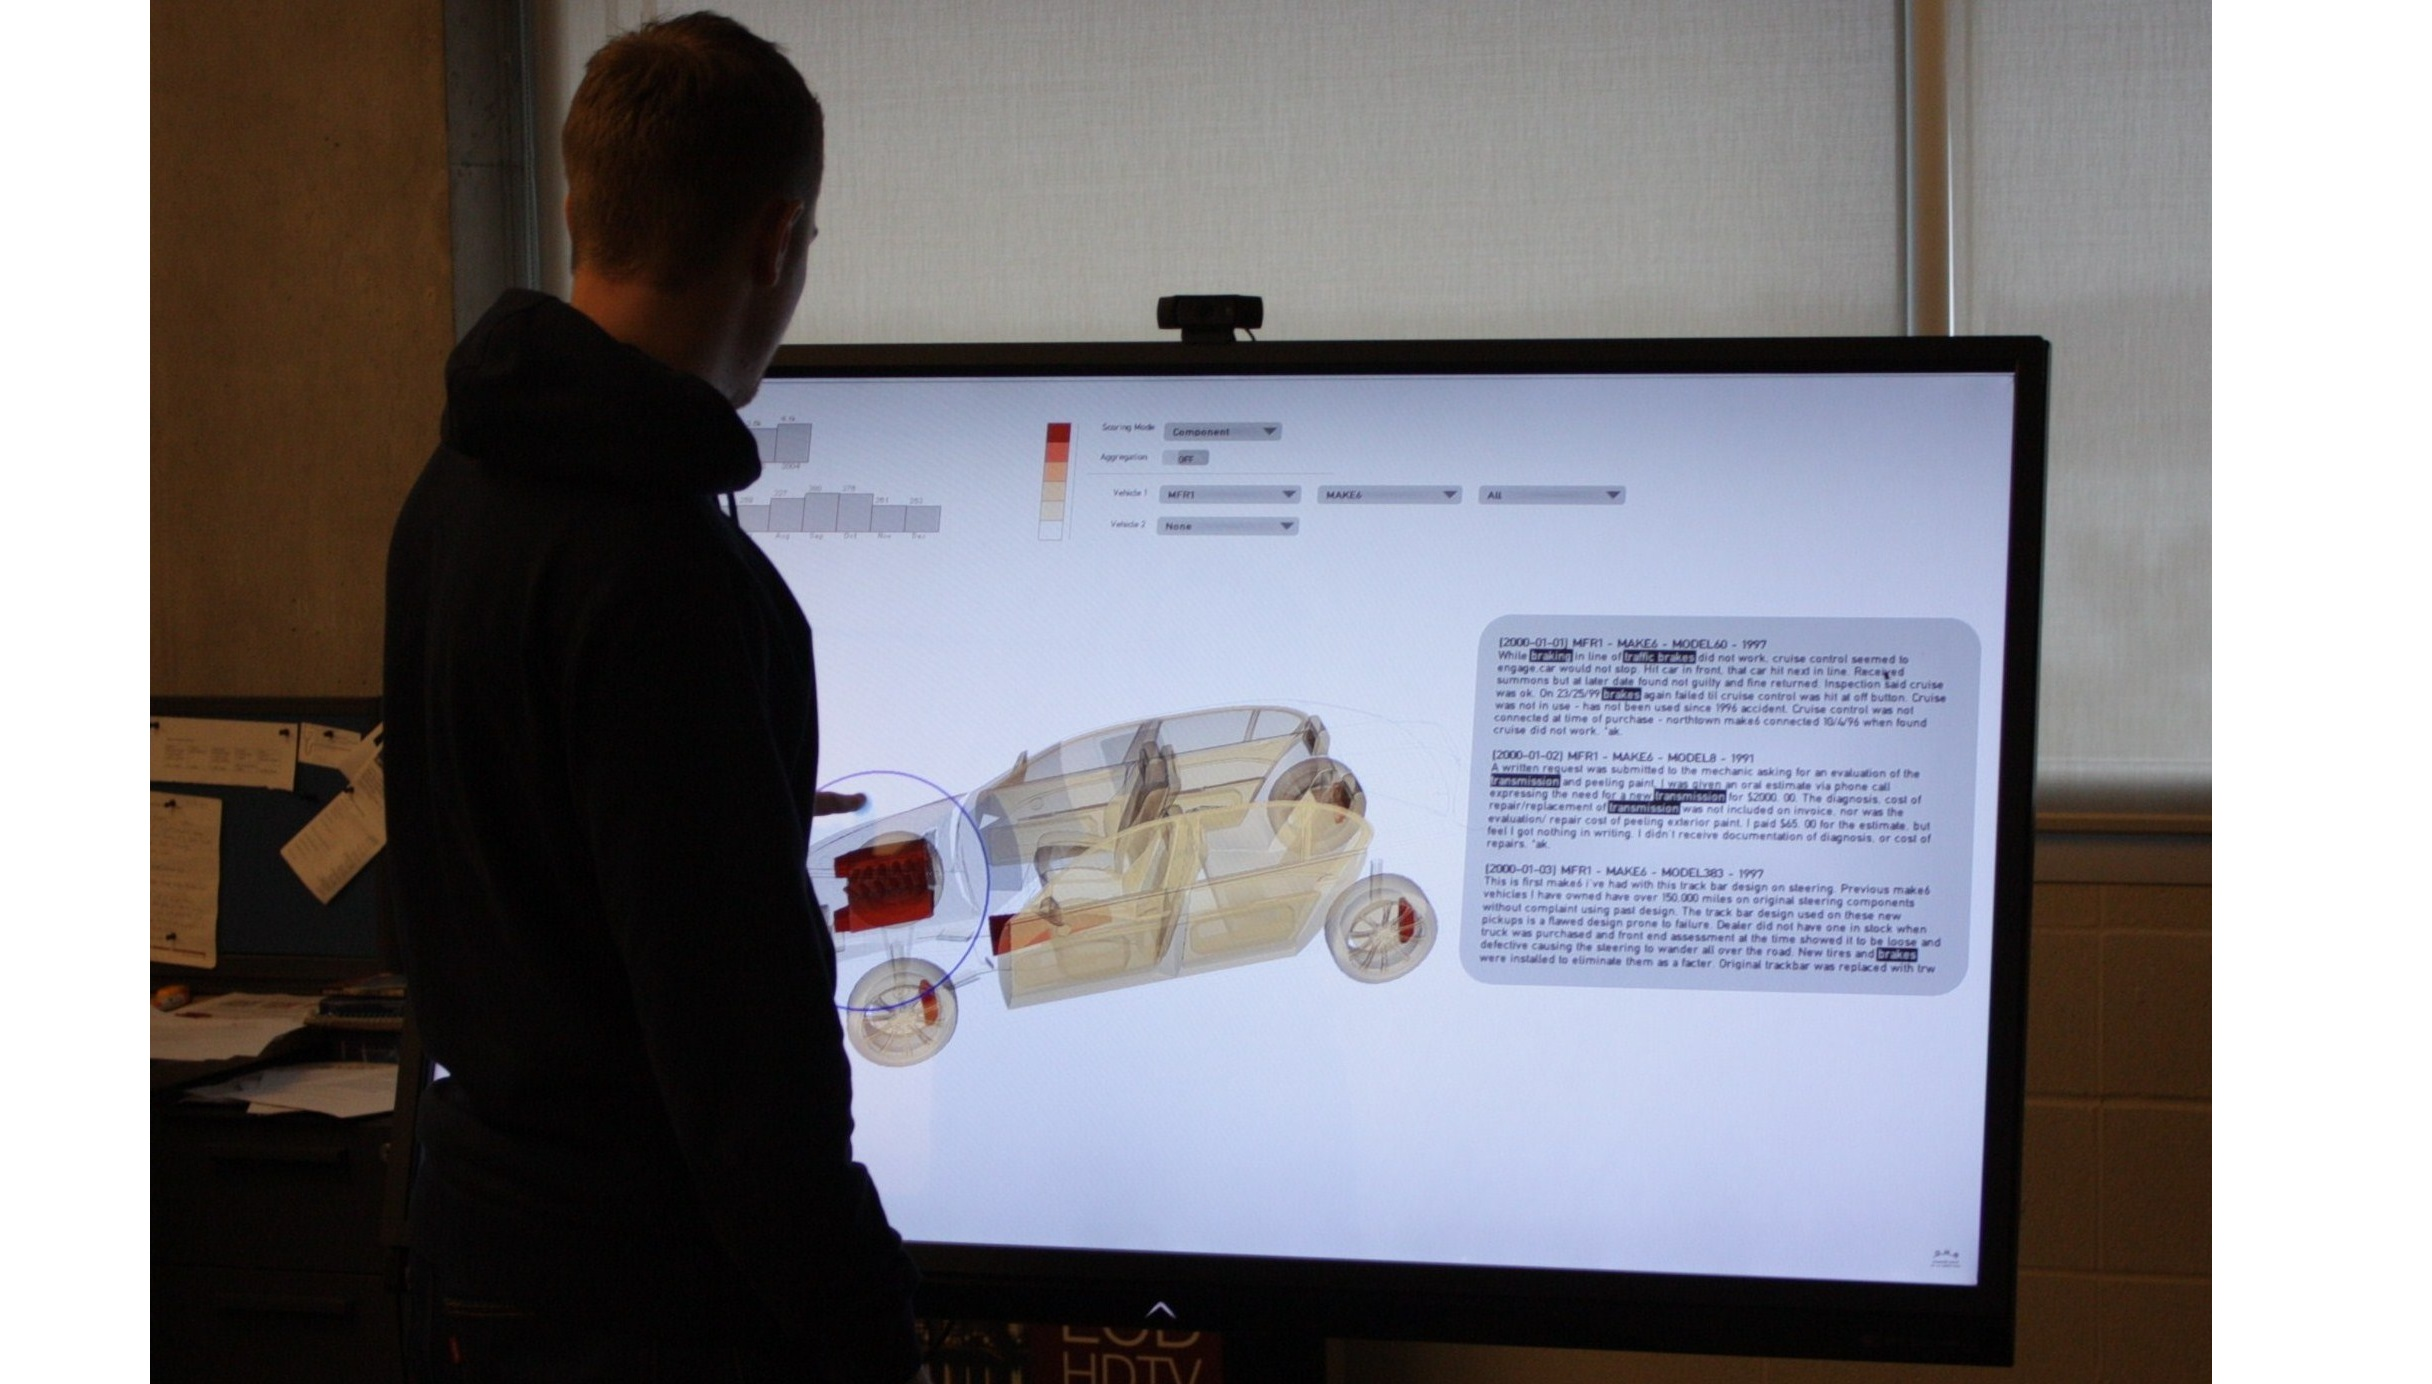
\includegraphics[width=\columnwidth]{erik_touch.JPG}  
	 \caption{Study setup.}
	 \label{figure:study}
	\end{figure}
	% ==============   


The study took place in a controlled lab environment. The visualization ran on
a 60 inch display fitted with a PQLabs infrared sensor overlay capable of
multitouch recognition. To avoid personal bias that may came from prior domain
knowledge, known identifiers were removed and replaced with placeholders.
For example the model ``Civic'' was replaced with ``Model1.'' The dataset for
the study itself includes the top four occurring manufacturers, and we used a time
frame between 1997 and 2004. Two pilot studies, both with lab members, were
conducted beforehand to ensure the study was appropriate, and allowed us to
tweak usability issues. Our setup can be seen in Figure \ref{figure:study}.

Each session was recorded on video, and touch interactions were
logged by the system. Each participant was compensated with a \$10 gift
certificate for their effort. Our complete study procedure can be found in Appendix A.


After a brief tutorial on how to interpret the visualization and how to use the
interface, participants were asked to perform three sets of tasks. The first set
consists of warm-up exercises aimed to help participants become familiar with the 
interactions (these are excluded from our analysis). Next came a set of
focused tasks with specific answers, they are intended to indicate whether the
\threed visualisation can be accurately perceived. For example, one question may
be ``Select the most complained about component in the year 1999.'' Finally,
the third set of questions is subjective in nature and has open-ended answers.
For these, we presented participants with a view of the data and asked them to
describe what they see, mentioning any trends or patterns, and lastly make a
decision based on a comparison of two vehicles. For example: ``Between 1997 and
2000, which of the vehicles X and Y would you purchase and why? Assume these vehicles are
similarly priced.'' All tasks were computer-based and pre-programmed into the system, 
the interface was reset automatically between tasks. After these tasks were completed, 
we conducted a semi-structured interview to solicit opinions from participants about their experiences.  

Each study session took approximately one hour to complete, though there were no
strict time constraints and participants were allowed to take as much time as
they wanted on any task. The same tasks were used for all
participants. 


\subsection{Data Collection}
In addition to written observations, video data and system log data were 
collected during the sessions. We used the video recordings to review 
participant's answers, in particular for the interview portions to verify 
our observations. Although not in scope of our study, the videos can also provide 
valuable implications for design, as they can show where and why participants had 
problems interacting with the system, we leave this as part of our future work. 

For the system logs, we tracked user input events that impact system states such
as changes to selections and data filters. We also tracked widget usages, when they were used and
their usage duration. The logs are used to reveal if there are any preferences and usage 
patterns.
 

% Consider rewriting this to be more specific at showing how rather than
% completion rates
\subsection{Discussion}
12 participants took part in the study, however one study session was excluded
from data analysis. The reason for the elimination was due to insufficient language skills; 
this participant had severe difficulty understanding the instructions of the tasks, 
and provided confusing and contradictory statements during the interview portion.


%Interpretation of the \threed visualization seemed to be fairly accurate for
%simple scenarios, while more complicated target acquisition tasks that required
%multiple steps yielded mixed results. The first two tasks asked
%participants to directly identify the mostly significant outliers, to accomplish
%these tasks, participants were to visually identify the outlier \threed
%component and select it. There were no restrictions on their method of
%selection. In total, 8/11 and 10/11 answered correctly, however, one participant
%who selected the incorrect entity later stated that the selection was based on
%personal opinion rather than a direct interpretation of the visualization.

In general, feedback of our visualization was favourable and most tasks were
completed reasonably well, in the sense that the conclusions drawn by the
participants were derived based on findings from using our system. There are a
few exceptions: some participants did not correctly respond to the focus
questions that asked them to identify outliers (3/11 and 1/11). This may partly
be attributed to initial unfamiliarity with what the visualization is trying to
show, as one participant (P5) revealed later that the first few answers were not
based on the visualization, but rather on personal opinion about automotive
vehicles. The other exception was the third task, which asked participants to identify
which of the four manufacturers used in the study had the highest engine
complaints. To complete the task, participants had to look at each
manufacturer one-by-one, or carry out a series pairwise comparisons to find the
maximum. We believe the complexity of having to memorize multiple states likely
contributed to the incorrect answers, in total five participants chose the correct
manufacturer. 

The interpretations of co-occurrence relationships were also mixed. In these
tasks, we asked the participants to identify the components that failed when
component X failed. We expected the participants to select X and then identify
the remaining entities in the visualization. However, we found that three participants
had difficulties understanding the co-occurrence concept. We are unsure whether
this is due to insufficient explanations at the start of the study, or the fact
that the same colouring scheme is used for both occurrence co-occurrence caused
the confusions. Somewhat unexpectedly, two participants noted that document
widget also shows co-occurrences in textual form, and read the documents
directly instead of using the \threed visualization.

Analysis of subjective tasks showed that participants generally had no problems
in accomplishing what was asked. For the task regarding trend analysis, most
attention was on the heatmap widgets. Five participants explicitly mentioned
outlier months in particular vehicle components over the twelve months period
that they found to be peculiar. three participants made note of possible seasonal trends,
such as winter months usually had higher number of complaints. The remaining three 
participants did not observe any specific patterns or outliers. 

For the comparison task of picking a reliable vehicle, the participants
focused on the \threed visualization. Six participants made the choice based on
preconceived notions of which components are more vital than others. For example,
some chose solely based on which vehicle had a lower rate of engine failures. Four
chose based on the sheer number of different components that failed. The
remaining lone participant was not able to make a choice but was able to
correctly interpret the visualization, mentioning each vehicle's problems
and that neither one was desirable. One participant did not directly use the
comparison function; rather each vehicle was examined one at a time.


 
% Usage data chart
% \begin{figure}
% \begin{tikzpicture}
% \begin{axis}[ 
%     width=13cm,
%     height=8cm,
%     bar width=0.2cm,  
%     ybar=0,
%     ymin=0,
%     symbolic x coords={P1, P2, P3, P4, P5, P6, P7, P8, P9, P10, P11},
%     xtick=data, 
%     legend style={at={(1.25, 0.9)}},
%     area legend,
%     ylabel=seconds
%     ] 
%     \addplot[ybar,fill=blue!75] 
%        coordinates { (P1,85) (P2,172)(P3,106) 
%                      (P4,5)  (P5,11) (P6,96)
%                      (P7,90) (P8,90) (P9,22)
%                      (P10,19) (P11,23)
%        }; 
%     \addplot[ybar,fill=red!25] 
%        coordinates { (P1,160) (P2,4)  (P3,169) 
%                      (P4,45)  (P5,83) (P6, 45) 
%                      (P7,0)   (P8,62) (P9,54)
%                      (P10,19) (P11,143)
%        };
%     \legend{Lens, 3D Scene}    
% \end{axis}
% \end{tikzpicture}
% \caption{Time spent on Lens and 3D Scene.}
% \label{chart:usage}     
% \end{figure}
%   
%    
% In terms of interaction with the system, we observed three different
% interaction styles. One group (P2, P7) used the lens almost exclusively
% as their primary navigational tool. The second group (P4, P5, P11) were the
% opposite and used direct manipulations to rotate and zoom the \threed model to
% access different components. The last group used a combination of both lens
% widget and direct manipulation. A chart showing the distributions of time spent
% on each widget can be see in Figure \ref{chart:usage}.

    % === Figure === 
	\begin{figure}
	 \centering  
	 \includegraphics[width=\columnwidth]{timechart5.png}  
	 \caption{Widget usage for the task of comparing two vehicles.}
	 \label{figure:timechart}
	\end{figure}
	% ============== 

In Figure \ref{figure:timechart}, we present a summary of the interaction logs
for the task of comparing two different types of vehicles. In this task
participants were free to use any widget they want to investigate which of the
two vehicles is more reliable. From the figure, we see that participants first
remove irrelevant data using the filters, then they either interact with 
the lens widget or directly with the \threed scene to explore the visualization.
The navigation actions were mostly executed in short bursts, followed by an idle
period. This behaviour appears to correspond to finding interesting data and
then spending time to asses his/her findings. We thought for most participants
the lens widget would be used only after the \threed model is moved into a
desired orientation, however this is not supported by the logs. The participant
strategies seem to group in to three types: use of both the \threed scene and
the lens widget for exploration (P3, 6, 8, 9, 10), only the lens widget (P2, 7),
and only the \threed scene (P1, 4, 5, 11). Surprisingly, participants did not
make use of the document during this task. Further investigation of the role of
full-text details can play in decision-making using d-NPR is warranted.


 
\subsection{Participant Feedback}
Participants enjoyed using the \threed visualization along with the lens widget.
Several participants made explicit comments with regards to the usage of a
familiar form factor through the \threed model. \emph{``Nicer to look at a
picture than a bunch of numbers.''} (P1), \emph{``everything is in detail, very
interactive.[\ldots] The visual, is self-explanatory''} (P8), \emph{``I can see
clearly each part in the car, so I know what to choose''} (P6), and \emph{``it is
relatable, I've been in cars and I've had the opportunity to see some of the
components.''} (P2). Using the lens widget for dynamic focusing of interesting
data was voiced by several participants: \emph{``kind of cool, being able to
dissect with it.''} (P1) and \emph{``You can zoom in to the parts that you
cannot really understand, for example the transmission.''} (P7).

Interaction with the heatmap had the most negative reactions. Four participants
thought the heatmap provided too much detail, they argued that an ordinary
consumer would not care for trend details, they would only care about the
overall verdict of whether a component is reliable or not. In particular, P11
suggested using a pie-chart or a bar-chart for each component in comparison view
rather than using a heatmap.  The design implication here may be to provide
different levels of granularity that can be dynamically adjusted. The lack of
labelling on the heatmap was raised by three others, as it made it more
difficult to identify individual months. Also the additional colour encoding
that is applied to the border of each cell in comparison mode made it more
difficult to distinguish the different severity levels. 

Overall, we observed several interaction issues. A few participants tried to
use the lens' depth function to access occluded objects, however we noted that
there were difficulties making fine adjustments, especially if the objects are
close to each other. Problems interacting with the touch surface was a general
concern voiced during the study, in particular we observed problems with
selection/deselection and manipulation of the filter widgets. The touch issues 
are exemplified in Figure \ref{figure:timechart}, note the time duration spent
on the filters, also note the rapid succession of selection actions which may
indicate problems with our multitouch heuristics. Despite these problems,
participants seem to enjoy using the visualization: \emph{``even though there
are some interaction problems, it just looks really good~``} (P10).

%The \threed visualization and lens mechanism received the most positive
%feedback. Participants liked how the \threed model can be used to provide 
%an overview showing all the entities. They also found it fun and enjoyed using
%the lens to focus in on specific regions, particularly for revealing objects
%that were unknown to them before.

%Interaction with the heatmap widget had the most negative reactions. Four
%participants thought the heatmap widget provided too much detail, they argued
%that an ordinary consumer would not care for trend details, they would only care
%about the overall verdict of whether a component is reliable or not. Three other
%participants had concerns about the readability of the heatmap itself, they
%mentioned that the lack of labelling made it difficult to identify individual
%months. Also the additional colour encoding that is applied to the border of each
%cell in comparison mode made it more difficult to distinguish the different
%severity levels. Several participants tried to use the lens' depth function to access
%occluded objects, however we observed that there were difficulties making fine
%adjustments, especially if the objects are close to each other. 
  
During the interview session, we asked the participants what they would do to
improve the system, there are four ideas relating to visualizations that emerged
from the study sessions:
\begin{itemize}[noitemsep]
  \item Non-consecutive years: Allow non-contiguous selection. For
  example select the years 2000 and 2002. Several participant also mentioned it
  would be nice to make year-to-year comparisons for each entity without
  leveraging the heatmap.
  
  \item Semantic zoom for the document widget: Several participant noted that
  the text on the document widget felt overwhelming, and would be better to
  present a brief summary before diving into the full text.
  
  \item Provide entity summary: The system only shows the name of the entity,
  there are a few participants that mentioned it would be nice to add a brief
  description to what the entity is and its function.
  
  \item Regional select: Provide a shortcut to select all entities under the
  lens.
\end{itemize}
   
  
\subsection{Summary}
Our study sessions showed that in general people were able to interpret the
visualization correctly. However for complicated situations where the analysis
require multiple steps, results tend to vary. In cases like this, a different
design approach such as supporting history or breadcrumb trails may be useful.
In the open-ended tasks, we observed that participants were able to use the
visualization and various interaction widgets to help guide their analysis.

The \threed visualization itself was intuitive. There are times where we did not
sufficiently explain the interface but participants were able to correctly infer
the correct interpretation. For example P1 was able to tell which entities had higher rate
of complaints in comparison mode even though we failed to mention the encoding scheme during demo. 
The semantic relations of occurrence and co-occurrence were harder to understand, which 
came as a surprise as we did not encounter comprehension issues in our pilot studies, 
perhaps a more hands-on tutorial would have helped.

%Performance???
Overall, the receptions of using the visualization were positive; other than the
comments above, \emph{``cool''}, \emph{``relatable''}, and \emph{``that
was really neat''} were heard through out the study sessions. However, as our
study is by large exploratory and qualitative in nature, a more thorough study
that involves more complex scenarios and performance metrics may further
validate the strength of our visualization approach.


%Overall, the receptions of using the visualization system were positive;
%comments such as ``cool,'' ``relatable,'' and ``that was really neat'' were heard
%through out the study sessions. Other comments, such as ``seeing all the different angles is
%nice'' and ``even though there are some interaction problems, it just looks
%really good!'' suggested the aesthetic value in showing a non-photorealistic \threed
%representation.  
  